\documentclass[aspectratio=169,9pt,t]{beamer}

\usepackage[T1]{fontenc}
\usepackage{lmodern}
\usepackage{amsmath,amssymb,mathtools}
\usepackage{tikz}
\usetikzlibrary{arrows.meta,positioning,calc,fit}

% This deck is a constructed teaching control.  It keeps the objective,
% graph, channel evidence, and initial point of lbfgs_three_bit_synced_deck.tex,
% but replaces L-BFGS by fixed-step projected gradient descent.

% ---------- palette and Beamer setup ----------
\definecolor{Ink}{HTML}{172033}
\definecolor{Muted}{HTML}{5F6B7A}
\definecolor{Canvas}{HTML}{FAFAF7}
\definecolor{Graph}{HTML}{77736B}
\definecolor{GD}{HTML}{087D77}
\definecolor{GDSoft}{HTML}{E5F5F2}
\definecolor{Gold}{HTML}{B85F00}
\definecolor{GoldSoft}{HTML}{FFF3D6}

\usetheme{default}
\usefonttheme{professionalfonts}
\setbeamertemplate{navigation symbols}{}
\setbeamercolor{normal text}{fg=Ink,bg=Canvas}
\setbeamercolor{frametitle}{fg=Ink,bg=Canvas}
\setbeamercolor{statebar}{fg=Ink,bg=GDSoft}
\setbeamercolor{countbar}{fg=Ink,bg=white}
\setbeamercolor{explain}{fg=Ink,bg=white}
\setbeamercolor{takeaway}{fg=Ink,bg=GoldSoft}
\setbeamercolor{retained}{fg=Ink,bg=GDSoft}
\setbeamercolor{temporary}{fg=Ink,bg=GoldSoft}
\setbeamersize{text margin left=6mm,text margin right=6mm}
\setbeamertemplate{frametitle}{%
  \vspace{.6mm}\insertframetitle\par
  \vspace{.2mm}{\color{Graph}\rule{\textwidth}{0.4pt}}\vspace{-2.2mm}}
\setbeamertemplate{footline}{%
  \leavevmode\hbox{%
    \begin{beamercolorbox}[wd=.84\paperwidth,ht=2.5ex,dp=1.1ex,leftskip=6mm]{normal text}%
      \fontsize{5.8}{6.6}\selectfont\color{Muted}%
      Persistent count includes fixed $\boldsymbol\ell$ and current $\mathbf{x}$; graph data and temporary arithmetic are excluded; synchronized slides do not imply equal arithmetic or complexity
    \end{beamercolorbox}%
    \begin{beamercolorbox}[wd=.16\paperwidth,ht=2.5ex,dp=1.1ex,rightskip=6mm plus 1fil]{normal text}%
      \fontsize{6.2}{7.0}\selectfont\color{Muted}%
      Slide \insertframenumber\ of \inserttotalframenumber
    \end{beamercolorbox}}}

% ---------- fixed slide grammar ----------
\newcommand{\countstrip}[2]{%
  \begin{columns}[T,onlytextwidth]
    \column{.705\textwidth}
      \begin{beamercolorbox}[rounded=true,sep=.62ex]{statebar}
        \fontsize{6.4}{7.0}\selectfont\textcolor{Muted}{\bfseries SYNC BEAT #1 OF 7 \;·\; STATE NOW}\par
        \vspace{.15ex}\scriptsize #2
      \end{beamercolorbox}
    \column{.275\textwidth}
      \begin{beamercolorbox}[rounded=true,sep=.52ex]{countbar}
        \fontsize{6.4}{7.0}\selectfont\textcolor{GD}{\bfseries PERSISTENT STATE VALUES}\par
        \fontsize{6.1}{6.8}\selectfont
        fixed $\boldsymbol\ell$: 3 \quad current $\mathbf{x}$: 3\par
        optimizer history: none \quad \textbf{total: 6}
      \end{beamercolorbox}
  \end{columns}\vspace{.6mm}}

\newcommand{\phase}[1]{%
  \centering\colorbox{GoldSoft}{\strut\scriptsize\bfseries\textcolor{Gold}{#1}}\par\vspace{.6mm}}

\newcommand{\callout}[1]{%
  \begin{beamercolorbox}[rounded=true,sep=.65ex]{explain}
    \scriptsize #1
  \end{beamercolorbox}}

\newcommand{\takeaway}[1]{%
  \vspace{.3mm}\begin{beamercolorbox}[wd=\textwidth,rounded=true,sep=.6ex]{takeaway}
    \centering\scriptsize\bfseries #1
  \end{beamercolorbox}}

% ---------- diagram vocabulary ----------
\tikzset{
  bit/.style={circle,draw=GD,fill=white,line width=1.15pt,minimum size=8.5mm,inner sep=0pt,font=\scriptsize\bfseries},
  check/.style={rectangle,draw=GD,fill=GDSoft,line width=1.15pt,minimum width=8.5mm,minimum height=7.5mm,rounded corners=1.3pt,inner sep=0pt,font=\scriptsize\bfseries},
  edge/.style={draw=Graph!55,line width=1.1pt},
  activeedge/.style={draw=GD!32,line width=3.1pt},
  dependency/.style={draw=GD,line width=1.8pt,dashed},
  valuechip/.style={fill=white,draw=GD,rounded corners=1.6pt,inner xsep=1.8pt,inner ysep=1pt,font=\fontsize{6.5}{7}\selectfont,text=Ink},
  tempchip/.style={fill=GoldSoft,draw=Gold,dashed,rounded corners=1.6pt,inner xsep=1.8pt,inner ysep=1pt,font=\fontsize{6.5}{7}\selectfont,text=Gold},
  flowretain/.style={draw=GD,fill=GDSoft,line width=1.1pt,rounded corners=2.5pt,minimum height=12mm,text width=35mm,align=center,font=\scriptsize},
  flowtemp/.style={draw=Gold,fill=GoldSoft,dashed,line width=1.1pt,rounded corners=2.5pt,minimum height=12mm,text width=35mm,align=center,font=\scriptsize},
  flowarrow/.style={draw=GD,line width=1.35pt,-{Stealth[length=2.5mm]}},
  looparrow/.style={draw=Gold,line width=1.25pt,-{Stealth[length=2.5mm]}}
}

\newcommand{\gdgraph}[3]{%
  \node[check] (A) at (-1.7,1.65) {$A$};
  \node[check] (B) at ( 1.7,1.65) {$B$};
  \node[bit] (b1) at (-3.0,0) {bit 1};
  \node[bit] (b2) at ( 0.0,0) {bit 2};
  \node[bit] (b3) at ( 3.0,0) {bit 3};
  \draw[edge] (A)--(b1);
  \draw[edge] (A)--(b2);
  \draw[edge] (B)--(b2);
  \draw[edge] (B)--(b3);
  \node[below=3.5mm of b1,font=\tiny] {$x_1=#1$};
  \node[below=3.5mm of b2,font=\tiny] {$x_2=#2$};
  \node[below=3.5mm of b3,font=\tiny] {$x_3=#3$};
}

\newcommand{\graphstart}{\begin{tikzpicture}[x=.92cm,y=.92cm]}
\newcommand{\graphend}{\end{tikzpicture}}

\begin{document}

% Slide 1 — synchronized with BP slide 1
\begin{frame}{Plain projected gradient descent in one loop}
  \countstrip{1}{\textbf{TEACHING CONTROL: }keep the teaching objective and starting point used in the L-BFGS deck, but replace its optimizer. Retain $\mathbf{x}^{(t)}$.}

  \phase{FREEZE $\mathbf{x}^{(t)}$ \quad $\longrightarrow$ \quad CALCULATE $\nabla J$ \quad $\longrightarrow$ \quad FIXED STEP $\eta=0.25$ \quad $\longrightarrow$ \quad PROJECT AND REPEAT}

  \begin{columns}[T,onlytextwidth]
    \column{.43\textwidth}
      \centering
      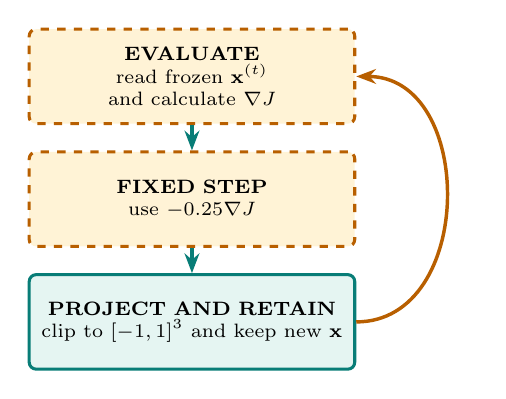
\begin{tikzpicture}[node distance=3.2mm]
        \node[flowtemp,text width=39mm] (eval)
          {\textbf{EVALUATE}\par read frozen $\mathbf{x}^{(t)}$ and calculate $\nabla J$};
        \node[flowtemp,text width=39mm,below=of eval] (direction)
          {\textbf{FIXED STEP}\par use $-0.25\nabla J$};
        \node[flowretain,text width=39mm,below=of direction] (move)
          {\textbf{PROJECT AND RETAIN}\par clip to $[-1,1]^3$ and keep new $\mathbf{x}$};
        \draw[flowarrow] (eval)--(direction);
        \draw[flowarrow] (direction)--(move);
        \draw[looparrow] (move.east) to[out=0,in=0,looseness=1.25] (eval.east);
      \end{tikzpicture}
    \column{.55\textwidth}
      \callout{\centering\textbf{Objective function in this teaching control}\par
        \[
          J(\mathbf{x})=-\frac12\sum_{i=1}^{3}\ell_i x_i
          +2\!\sum_{c\in\{A,B\}}\!\left(1-\prod_{j\in c}x_j\right)^2
        \]}
      \vspace{.7mm}
      \callout{\centering\textbf{One update}\par
        \[
          \mathbf{x}^{(t+1)}=\Pi_{[-1,1]^3}
          \!\left(\mathbf{x}^{(t)}-0.25\nabla J(\mathbf{x}^{(t)})\right)
        \]
        No $\mathbf{H}_t$, no $(\mathbf{s},\mathbf{y})$ pairs, and no line search.\par
        \vspace{.5mm}\fontsize{6.3}{7.0}\selectfont
        Constructed fixed-step control; not the retained native projected-GD endpoint.}
  \end{columns}

\end{frame}

% Slide 2 — synchronized with BP slide 2
\begin{frame}{Initialize once: channel evidence and one scalar per bit}
  \countstrip{2}{\textbf{INITIAL VALUES: }store fixed $\boldsymbol\ell=-\mathbf{L}$ and initialize $\mathbf{x}^{(0)}=\tanh(\boldsymbol\ell/2)$. There is no optimizer history.}

  \phase{PLACE FIXED $\boldsymbol\ell$ \quad $\longrightarrow$ \quad INITIALIZE $\mathbf{x}^{(0)}$ \quad $\longrightarrow$ \quad KEEP ONE SCALAR PER BIT}

  \begin{columns}[T,onlytextwidth]
    \column{.58\textwidth}
      \centering
      \graphstart
        \gdgraph{+0.800}{-0.200}{-0.333}
        \node[below=8.2mm of b1,font=\tiny,text=Muted] {$\ell_1=+2.197$};
        \node[below=8.2mm of b2,font=\tiny,text=Muted] {$\ell_2=-0.405$};
        \node[below=8.2mm of b3,font=\tiny,text=Muted] {$\ell_3=-0.693$};
      \graphend
    \column{.40\textwidth}
      \callout{\centering
        \[
          \boldsymbol\ell=-\mathbf{L}
          =(+2.197,-0.405,-0.693)
        \]
        \[
          \mathbf{x}^{(0)}=\tanh(\boldsymbol\ell/2)
          =(+0.800,-0.200,-0.333)
        \]}
      \vspace{1mm}
      \begin{beamercolorbox}[rounded=true,sep=.75ex]{retained}
        \scriptsize\textcolor{GD}{\bfseries PERSISTENT NUMERICAL VALUES}\par\vspace{.4mm}
        \fontsize{7.2}{8.2}\selectfont
        fixed $\boldsymbol\ell[3]$ \hfill 3\par
        current $\mathbf{x}^{(0)}[3]$ \hfill 3\par
        optimizer history \hfill none\par
        \textbf{persistent total} \hfill \textbf{6}
      \end{beamercolorbox}
  \end{columns}

  \takeaway{Here $\ell_i>0$ and $x_i>0$ favour bit 0; the BP deck uses the opposite-sign channel LLR $L_i=-\ell_i$.}
\end{frame}

% Slide 3 — synchronized with BP slide 3
\begin{frame}{Frozen-state read: both checks calculate their residuals}
  \countstrip{3}{\textbf{LOCKED READ: }checks $A$ and $B$ read one frozen $\mathbf{x}^{(0)}$. The residuals are temporary; no coordinate changes during this slide.}

  \phase{LOCK $\mathbf{x}^{(0)}$ \quad $\longrightarrow$ \quad $A$ READS $x_1,x_2$ \quad + \quad $B$ READS $x_2,x_3$ \quad $\longrightarrow$ \quad CALCULATE $r_A,r_B$}

  \begin{columns}[T,onlytextwidth]
    \column{.58\textwidth}
      \centering
      \graphstart
        \gdgraph{+0.800}{-0.200}{-0.333}
        \draw[activeedge] (A)--(b1); \draw[activeedge] (A)--(b2);
        \draw[activeedge] (B)--(b2); \draw[activeedge] (B)--(b3);
        \draw[dependency] (A)--(b1); \draw[dependency] (A)--(b2);
        \draw[dependency] (B)--(b2); \draw[dependency] (B)--(b3);
        \node[draw=Gold,circle,line width=1.5pt,minimum size=11mm,fit=(b2),inner sep=0pt] {};
        \node[tempchip,above=5mm of A] {$r_A=1.160$};
        \node[tempchip,above=5mm of B] {$r_B=0.933333$};
      \graphend
    \column{.40\textwidth}
      \callout{\centering
        \[
          r_c=1-\prod_{j\in c}x_j
        \]}
      \vspace{.8mm}
      \callout{\centering
        $\begin{aligned}
          r_A&=1-(0.800)(-0.200)=1.160,\\
          r_B&=1-(-0.200)(-0.333333)=0.933333.
        \end{aligned}$}
      \vspace{.8mm}
      \begin{beamercolorbox}[rounded=true,sep=.65ex]{takeaway}
        \centering\scriptsize\bfseries
        Showing $A$ before $B$ is presentation order. Both calculations use the frozen vector.
      \end{beamercolorbox}
  \end{columns}

  \takeaway{The dashed lines show mathematical dependence on the coordinates; they do not show travelling messages.}
\end{frame}

% Slide 4 — synchronized with BP slide 4
\begin{frame}{Each check contributes terms to the gradient}
  \countstrip{4}{\textbf{ONE FROZEN SNAPSHOT: }all four $g_{c,i}$ terms use $\mathbf{x}^{(0)}$. They are indexed by check and coordinate only while $\nabla J$ is calculated.}

  \phase{READ FROZEN $\mathbf{x}^{(0)}$ AND $r_c$ \quad $\longrightarrow$ \quad CALCULATE FOUR $g_{c,i}$ TERMS \quad $\longrightarrow$ \quad KEEP $\mathbf{x}^{(0)}$ FIXED}

  \begin{columns}[T,onlytextwidth]
    \column{.58\textwidth}
      \centering
      \graphstart
        \gdgraph{+0.800}{-0.200}{-0.333}
        \draw[activeedge] (A)--(b1); \draw[activeedge] (A)--(b2);
        \draw[activeedge] (B)--(b2); \draw[activeedge] (B)--(b3);
        \node[tempchip] at ($(A)!.53!(b1)+(-.15,.05)$) {$g_{A,1}$};
        \node[tempchip] at ($(A)!.53!(b2)+(-.12,.05)$) {$g_{A,2}$};
        \node[tempchip] at ($(B)!.53!(b2)+(.12,.05)$) {$g_{B,2}$};
        \node[tempchip] at ($(B)!.53!(b3)+(.15,.05)$) {$g_{B,3}$};
      \graphend
    \column{.40\textwidth}
      \callout{\centering
        \[
          g_{c,i}=-4r_c\!\!\prod_{\substack{j\in c\\j\ne i}}\!x_j
        \]}
      \vspace{.7mm}
      \begin{columns}[T,onlytextwidth]
        \column{.49\textwidth}
          \callout{\centering\textbf{check $A$}\par
            $\begin{aligned}
              g_{A,1}&=+0.928,\\
              g_{A,2}&=-3.712
            \end{aligned}$}
        \column{.49\textwidth}
          \callout{\centering\textbf{check $B$}\par
            $\begin{aligned}
              g_{B,2}&=+1.244,\\
              g_{B,3}&=+0.747
            \end{aligned}$}
      \end{columns}
      \vspace{.7mm}
      \callout{\centering The four terms are temporary. They are combined by bit coordinate on the next slide.}
  \end{columns}

  \takeaway{The values contribute to the gradient of the objective function; they are not directed BP messages.}
\end{frame}

% Slide 5 — synchronized with BP slide 5
\begin{frame}{One sum per coordinate: GD has no recipient exclusion}
  \countstrip{5}{\textbf{AGGREGATE ONLY: }$\mathbf{x}^{(0)}$ remains frozen while every applicable term is added into one gradient coordinate. No outgoing check address is created.}

  \phase{GROUP TERMS BY BIT INDEX \quad $\longrightarrow$ \quad SUM EVERY APPLICABLE TERM \quad $\longrightarrow$ \quad FORM ONE $\partial J/\partial x_i$ PER BIT}

  \begin{columns}[T,onlytextwidth]
    \column{.45\textwidth}
      \centering
      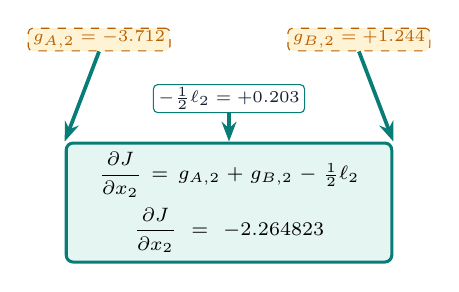
\begin{tikzpicture}
        \node[tempchip] (ga) at (-1.65,1.35) {$g_{A,2}=-3.712$};
        \node[tempchip] (gb) at ( 1.65,1.35) {$g_{B,2}=+1.244$};
        \node[valuechip] (ch) at (0,.60) {$-\tfrac12\ell_2=+0.203$};
        \node[flowretain,text width=39mm] (sum) at (0,-.72)
          {$\displaystyle \frac{\partial J}{\partial x_2}=g_{A,2}+g_{B,2}-\tfrac12\ell_2$\\[1mm]
           $\displaystyle \frac{\partial J}{\partial x_2}=-2.264823$};
        \draw[flowarrow] (ga.south)--(sum.north west);
        \draw[flowarrow] (gb.south)--(sum.north east);
        \draw[flowarrow] (ch.south)--(sum.north);
      \end{tikzpicture}
    \column{.53\textwidth}
      \callout{\centering\textbf{Complete gradient at the frozen point}\par
        \[
          \nabla J(\mathbf{x}^{(0)})=
          \begin{bmatrix}
            g_{A,1}-\tfrac12\ell_1\\
            g_{A,2}+g_{B,2}-\tfrac12\ell_2\\
            g_{B,3}-\tfrac12\ell_3
          \end{bmatrix}
          =\begin{bmatrix}
            -0.170612\\[-.3mm]
            -2.264823\\[-.3mm]
            +1.093240
          \end{bmatrix}
        \]}
      \vspace{.7mm}
      \begin{beamercolorbox}[rounded=true,sep=.75ex]{retained}
        \scriptsize\textcolor{GD}{\bfseries WHY THIS DIFFERS FROM BP SLIDE 5}\par\vspace{.5mm}
        Bit 2 receives terms associated with both checks $A$ and $B$. GD adds them into one coordinate $\nabla_2J$. It does not remove a recipient's contribution because it is not preparing an addressed message.
      \end{beamercolorbox}
  \end{columns}

  \takeaway{All applicable terms become one coordinate update; only the resulting $x_2$ can cross the next iteration boundary.}
\end{frame}

% Slide 6 — synchronized with BP slide 6
\begin{frame}{Move once: the next evaluation still has one bit-2 scalar}
  \countstrip{6}{\textbf{START: }$\mathbf{x}^{(0)}$ and $\nabla J(\mathbf{x}^{(0)})$. \textbf{END: }project the fixed step and retain $\mathbf{x}^{(1)}$; the temporary terms are discarded.}

  \phase{NEGATIVE GRADIENT \quad $\longrightarrow$ \quad FIXED STEP $0.25$ \quad $\longrightarrow$ \quad PROJECT TO $[-1,1]^3$ \quad $\longrightarrow$ \quad RETAIN $\mathbf{x}^{(1)}$}

  \begin{columns}[T,onlytextwidth]
    \column{.47\textwidth}
      \callout{\centering
        \[
          -\nabla J(\mathbf{x}^{(0)})
          =(+0.170612,+2.264823,-1.093240)
        \]
        \[
          \begin{aligned}
          \mathbf{z}^{(0)}
            &=\mathbf{x}^{(0)}-0.25\nabla J(\mathbf{x}^{(0)})\\
            &=(+0.842653,+0.366206,-0.606643),\\
          \mathbf{x}^{(1)}&=\Pi_{[-1,1]^3}(\mathbf{z}^{(0)})=\mathbf{z}^{(0)}.
          \end{aligned}
        \]}
      \vspace{.7mm}
      \begin{beamercolorbox}[rounded=true,sep=.65ex]{temporary}
        \centering\scriptsize
        $J(\mathbf{x}^{(0)})=3.398461$ \quad $\longrightarrow$ \quad
        $J(\mathbf{x}^{(1)})=2.881689$\par
        No coordinate is clipped on this step.
      \end{beamercolorbox}
    \column{.51\textwidth}
      \centering
      \graphstart
        \gdgraph{+0.843}{+0.366}{-0.607}
        \draw[activeedge] (A)--(b2); \draw[activeedge] (B)--(b2);
        \draw[dependency] (A)--(b2); \draw[dependency] (B)--(b2);
        \node[draw=Gold,circle,line width=1.6pt,minimum size=11mm,fit=(b2),inner sep=0pt] {};
        \node[valuechip,above=5mm of A] {$A$ next reads $x_2^{(1)}$};
        \node[valuechip,above=5mm of B] {$B$ next reads $x_2^{(1)}$};
        \node[font=\large\bfseries,text=GD] at (0,1.65) {$=$};
      \graphend
  \end{columns}

  \takeaway{Both checks next read the one retained $x_2^{(1)}$. This first point matches the teaching L-BFGS path because its empty-history direction is $-\nabla J$ and its line search accepts $\alpha=0.25$; later directions need not agree.}
\end{frame}

% Slide 7 — synchronized with BP slide 7
\begin{frame}{What crosses a plain projected-GD iteration boundary}
  \countstrip{7}{\textbf{AFTER THE STEP: }fixed $\boldsymbol\ell$ and current $\mathbf{x}^{(1)}$ remain. Residuals, $g_{c,i}$ terms, $\nabla J$, and the trial point are recalculated.}

  \phase{KEEP FIXED $\boldsymbol\ell$ AND CURRENT $\mathbf{x}$ \quad $\longrightarrow$ \quad RECALCULATE TEMPORARY TERMS \quad $\longrightarrow$ \quad PROJECT THE NEXT FIXED STEP}

  \begin{columns}[T,onlytextwidth]
    \column{.45\textwidth}
      \centering
      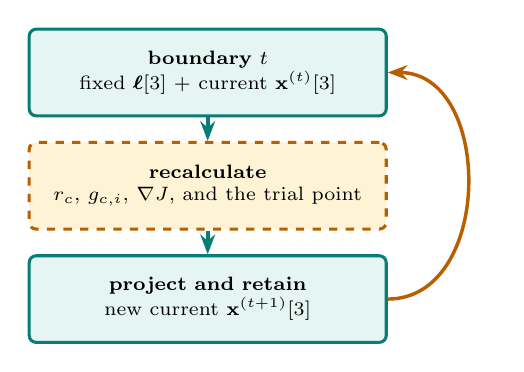
\begin{tikzpicture}[node distance=3mm]
        \node[flowretain,text width=43mm,minimum height=11mm] (boundary)
          {\textbf{boundary $t$}\\fixed $\boldsymbol\ell[3]$ + current $\mathbf{x}^{(t)}[3]$};
        \node[flowtemp,text width=43mm,minimum height=11mm,below=of boundary] (work)
          {\textbf{recalculate}\\$r_c$, $g_{c,i}$, $\nabla J$, and the trial point};
        \node[flowretain,text width=43mm,minimum height=11mm,below=of work] (next)
          {\textbf{project and retain}\\new current $\mathbf{x}^{(t+1)}[3]$};
        \draw[flowarrow] (boundary)--(work);
        \draw[flowarrow] (work)--(next);
        \draw[looparrow] (next.east) to[out=0,in=0,looseness=1.20] (boundary.east);
      \end{tikzpicture}
      \vspace{1mm}
      \begin{beamercolorbox}[rounded=true,sep=.8ex]{temporary}
        \centering\scriptsize
        The objective decrease on this toy update demonstrates the calculation only; it does not establish decoding performance.
      \end{beamercolorbox}
    \column{.53\textwidth}
      \begin{beamercolorbox}[rounded=true,sep=.8ex]{retained}
        \scriptsize\textcolor{GD}{\bfseries PERSISTENT AFTER THE FIRST STEP}\par\vspace{.5mm}
        \fontsize{7.2}{8.3}\selectfont
        fixed channel evidence $\boldsymbol\ell$ \hfill 3 values\par
        current relaxed vector $\mathbf{x}^{(1)}$ \hfill 3 values\par
        optimizer history \hfill none\par\vspace{.6mm}
        \textbf{persistent total} \hfill \textbf{6 values}
      \end{beamercolorbox}
      \vspace{1mm}
      \begin{beamercolorbox}[rounded=true,sep=.8ex]{temporary}
        \scriptsize\textcolor{Gold}{\bfseries RECALCULATED, NOT RETAINED}\par\vspace{.5mm}
        $r_A,r_B$; four $g_{c,i}$ terms; $\nabla J$; negative-gradient step; raw proposal and reusable projection workspace.\par\vspace{.5mm}
        A concrete implementation needs reusable working storage. Its peak depends on the chosen evaluation schedule, so six is a persistent-state count, not a universal memory bound.
      \end{beamercolorbox}
      \vspace{1mm}
      \callout{\centering\textbf{Mechanism contrast}\par
        BP retains separately addressed edge messages. This projected-GD control retains one scalar $x_i$ per bit.}
  \end{columns}

\end{frame}

\end{document}
